\section{Introduction}
MultiProcessor System on Chips (MPSoCs) have significantly proliferated in the embedded system domain due to the scaling of transistor. Furthermore, the MPSoCs can be configured to satisfy the requirements of the target applications, leading to an Application Specific MPSoC. The cores in Application Specific MPSoC can be diverse in nature and may include coprocessors, DSPs,  general purpose processors or hardware accelerators. The heterogeneity in designing Application Specifc MPSoC can be exploited to improve the efficiency of parameters like performance, area and energy consumption for the target application.

Low energy consumption is highly desirable for MPSoCs that are used in portable devices to increase the battery life of the device. Prior research has shown that the use of Dynamic Voltage and Frequency Scaling (DVFS) and customization of the processors are two effective techniques for reduction of energy consumption ~\cite{energy_asip}. This is particularly so for
streaming applications, which contain sub-kernels that are executed
repeatedly in a pipelined fashion~\cite{pipeline}. DVFS results in quadratic
reduction in energy with only linear sacrifice of the processor speed.
Streaming applications benefit from DVFS by exploiting the slack of non-
critical stages to reduce their dynamic energy consumption.

Customization of the processors in an MPSoC is typically achieved through
the use of Application Specific Instruction set Processors (ASIPs) ~\cite{sun_asip}.
ASIPs can be customized according to the sub-kernels of a streaming
application. The addition of custom instructions to an ASIP improves it's
energy efficiency for the following reasons: the number of instruction
fetches reduces, and the number of register file accesses for data
transfer between the instructions reduces ~\cite{energy_custom}. On the other hand,
custom instructions can also have a detrimental effect because of the
increase in on-chip area, and thus in the leakage energy consumption.
Hence, a designer has to carefully choose custom instructions to minimze
the energy consumption. 

In an ASIP, the memory subsystem (caches) contributes significantly to
its total energy consumption ~\cite{mem_en1, mem_en2}. In particular, the memory subsystem
is a significant contributor of the on-chip area, and thus of the total
leakage energy consumption. Therefore, design of a memory subsystem
is also crucial in improving not only the energy efficiency, but also
the performance and the area utilization of an ASIP. Existing works on
reducing energy consumption in the memory subsystems are~\cite{mem_en2}. 

Traditionally, researchers have focussed on reducing energy consumption
of ASIP based MPSoCs with the addition of custom instructions or
customization of the cache or the use of DVFS. They fail to consider
all the three techniques together for maximal reduction in energy
consumption. With the customization of the ASIPs and their caches, and
the added advantage of DVFS, one can synergistically design an energy-
efficient heterogeneous MPSoC for streaming applications, which are the
basis of entertainment in portable devices~\ref{}.

\begin{figure}[h]
\label{fig:motivation}
\center
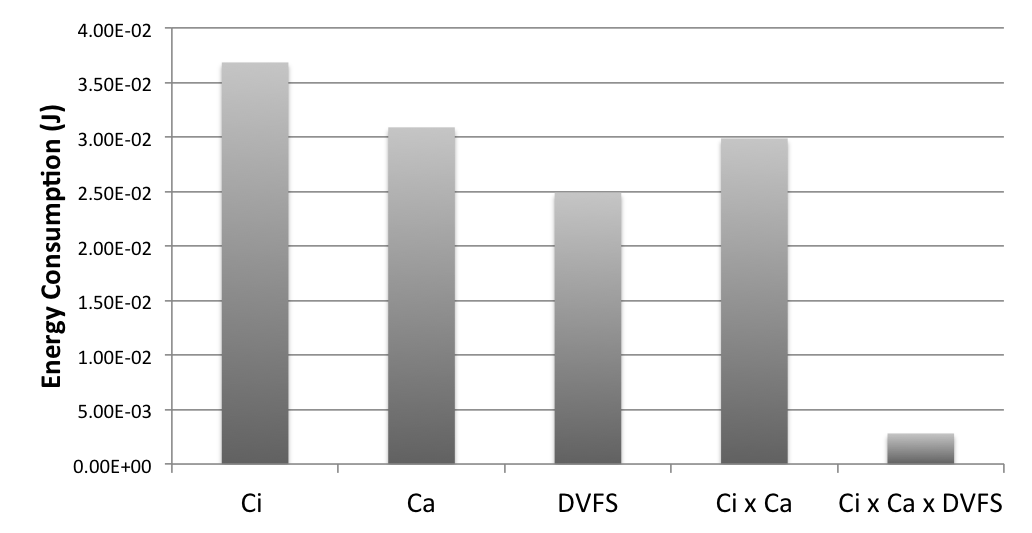
\includegraphics[width=0.40\textwidth]{motivation.png}
\caption {Minimal Energy Consumption for DCT kernel of MP3 encoder}
\end{figure}

To show the importance of considering all the three techniques
together, we analyze a sub-kernel of a streaming application. We
chose \textit{discrete cosine transform (DCT)} sub-kernel from the
\textit{MP3} encoder application. The experimental setup is described
in detail in Section~\ref{}. Figure~\ref{} plots the minimal energy
consumption achievable for each of the following techniques: a) Only custom instructions are added (\textbf{Ci}), b) Only cache
is customized (\textbf{Ca}), c) Only DVFS is used (\textbf{DVFS}
) d) Custom instructions are added with customization of the cache
(\textbf{Ci $\times$ Ca}) and e) All the three techniques are considered
simultaneously (\textbf{Ci $\times$ Ca $\times$ DVFS}). Use of both the
custom instructions and customized cache is better than their individual
use because addition of custom instructions modifies a kernel’s behaviour
such as code size, data transfers between instructions, memory access
pattern, etc. Therefore, a designer should choose an appropriate cache
based on the custom instructions to improve the energy efficiency. Next,
the use DVFS, in addition to custom instructions and customized cache,
results in minimum energy consumption, which is significantly lower than
the other techniques. Thus, it is evident that separate use of the three
energy reduction techniques may result in a local optima. Therefore, it
is desirable to use all the three techniques together to reach better
global optima.

Although the use of custom instructions, customized cache and DVFS
achieves better energy efficiency, their combined use significantly
increases the complexity of the optimization problem. For instance,
consider an application with only four tasks, four different custom
instructions per task, four different voltage/frequency levels and four
different cache configurations. Then, the total number of points in the
design space is more than a billion. Therefore, in this paper, we focus
on the problem of selecting custom instructions, cache configuration and
voltage/frequency level for sub-kernels of a streaming application, which
is executed on an MPSoC. To aid quick and efficient exploration of the
design space, first we propose estimation methods to compute execution
time and energy consumption of a sub-kernel. Then, we design a novel
branch and bound algorithm to efficiently prune and search the design
space. In particular, this paper has the following contributions:

\begin{enumerate}

\item We propose a novel problem formulation for ASIP systhesis based on
energy efficiency.

\item We develop an analytical framework to explore the complex design
space involving custom instruction set versions, cache sizes and voltage/
frequency settings simultaneously.

\item We propose a novel branch and bound algorithm to identify the
optimal points in the complex design space.

\item Finally, we compare our technique with the exisiting conventional
techniques for energy optimization.

\end{enumerate}